\chapter{Evaluation}
The system was tested with manual and automated functionality test. These tests have also given some information about performance, reliability and correctness. Evaluating a system, which takes baby steps into a completely new environment, was quiet challenging. Since most of the work consisted of coming up with the concepts and architecture, the implementation is somewhat chaotic and often not best practice oriented as in the Implementation chapter. Nevertheless, the code has been tested and important conclusions were drawn.
\section{Testing Environment}
\begin{figure}
    \centering
    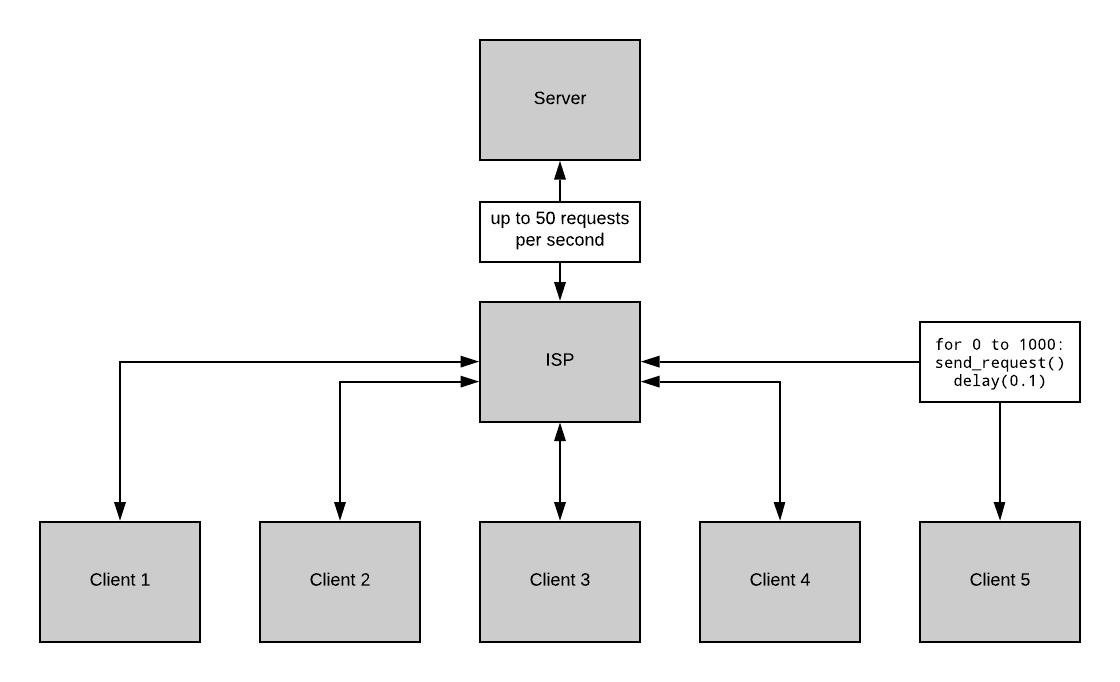
\includegraphics[width=\textwidth]{tests}
    \caption{Testing setup.}
    \label{fig:tests}
\end{figure}
As seen in the implementation section, the client can call services via requests from the ISP, as well as from the server, after introducing itself. Given this, the main testing aspect was to see that the ISP and servers can keep up with the work load and distribute the results back to their origins. The test was conducted as follows:\\
First, the implementation was tested manually by testing each functionality on its own. Second, the automated test was conducted. At the beginning, there were three nodes involved, one client, one ISP and one server. After initialising all nodes, the client went into a loop, where it first introduced itself to the server. The server automatically accepted this request and the feed-pair was created. After this, a random number was created between 5 and 20, which was the amount of service requests sent to the now connected server. To mimic a human interaction, delays of between the 1.0 and 4.0 seconds were used at first, randomly distributed with one decimal place between the RPC-requests. This was the basic evaluation of functionality, performance, reliability and correctness.\\
Unfortunately, after approximately 50 requests, either the ISP or the server had an exception on the cbor2 library\footnote{cbor2 5.1.0 - \url{https://pypi.org/project/cbor2/} - retrieved 02.07.2020} . Something with the bytestream seemed to be broken. Any other solution than just ignoring this exception and leaving this specific log entry hanging could not be found. This resulted in an open, unresolved request which the client waited for. \\
In a next step, after ignoring inconsistencies in the log entries, the system was tested to its limits, by having delays lowest at 0.1 seconds, adding more and more clients and up to a thousand iterations per client. My personal machine nearly broke down during the last test with a delay of 0.1 seconds, 5 clients and a combined one thousand requests per client. The tests lead to interesting results.

\section{Results}
\subsection{Functionality}
The functionality was tested manually on different Linux distributions\footnote{Ubuntu - 18.04.4 LTS, Python 3.6.9}\footnote{Ubuntu - 19.10, Python 3.7.5}\footnote{Arch - 5.7.6, Python 3.8.3} where as on Windows and Mac OS, serious problems occurred. The file system monitor\footnote{Watchdog for Python - \url{https://pythonhosted.org/watchdog/} - retrieved 30.06.2020} could not detect any changes on feeds, even when they were made. As far as concerned and tested on Linux distributions, the functionality is complete, the whole process of requesting services from the ISP, as well as introducing to different servers, is given and works as intended. This is the case only when the user strictly follows the documentation on how the system must be used. The user experience is not particularly intuitive and wrong use can corrupt the system. This as found in a very early stage of the project, but by iterating over it, these issues can be found and eliminated.
\subsection{Performance}
The performance begins with an astonishing speed, with nearly no latency between request and response, but collapses over time. This fact was already known at the implementation point. To distinguish between already handled and completed requests, the system cycles through the whole feed every time a change is detected. This problem can be solved by indexing the feed and saving the previously reached position. This factor has been left out intentionally to concentrate on the underlying concepts and architecture of the big 
picture.
\subsection{Reliability and Correctness}
As already indicated in the section Testing Environment, some \textit{undefined} or \textit{undiscovered} fault between this implementation and the cbor2 library\footnote{cbor2 5.1.0 - \url{https://pypi.org/project/cbor2/} - retrieved 02.07.2020} caused some ignore requests. Having this information, the tradeoff between the reliability and correctness of the feed-bundle protocol is obvious. Having the underlaying simplified RPC protocol, the fact that request do not get a response violates the consensus given by \citet{birrell1984implementing}. If it is not exactly specified, this does not line out a huge problem, but in order to achieve a fully functional system, some sort of error detection must be given. This error detection must find such "log entry loss" and resend the requests. Consequential, all these findings generalise one big problem.

\subsection{General Collaboration of Components}
Due to the fact that this completely new technology was developed in just a few months, with a focus on the general aspects, a patchwork of different libraries, common technologies and new technologies, which are not coordinated with each other, is the result. To generally improve the very broadly open architecture and procedures need to be tightened, with more rules and less freedom, resulting in a more specific implementation where the components are written to function optimally with each other.  The claim in this thesis that the onboarding experience is made easier has definitely been shown. After establishing a contract with an ISP on start-up of the software the client is directly connected to this ISP and indirectly connected to the  servers the ISP holds contracts with. However, the hypothesis that by splitting the ID-centric feeds from Secure Scuttlebutt into feed-pairs bundled by the Feed Bundle Protocol, the load on the wire can be reduced, can not yet be judged. The Feed Bundle Protocol is in a preliminary stage, with not enough experience in its implementation, to achieve that kind of judgement.